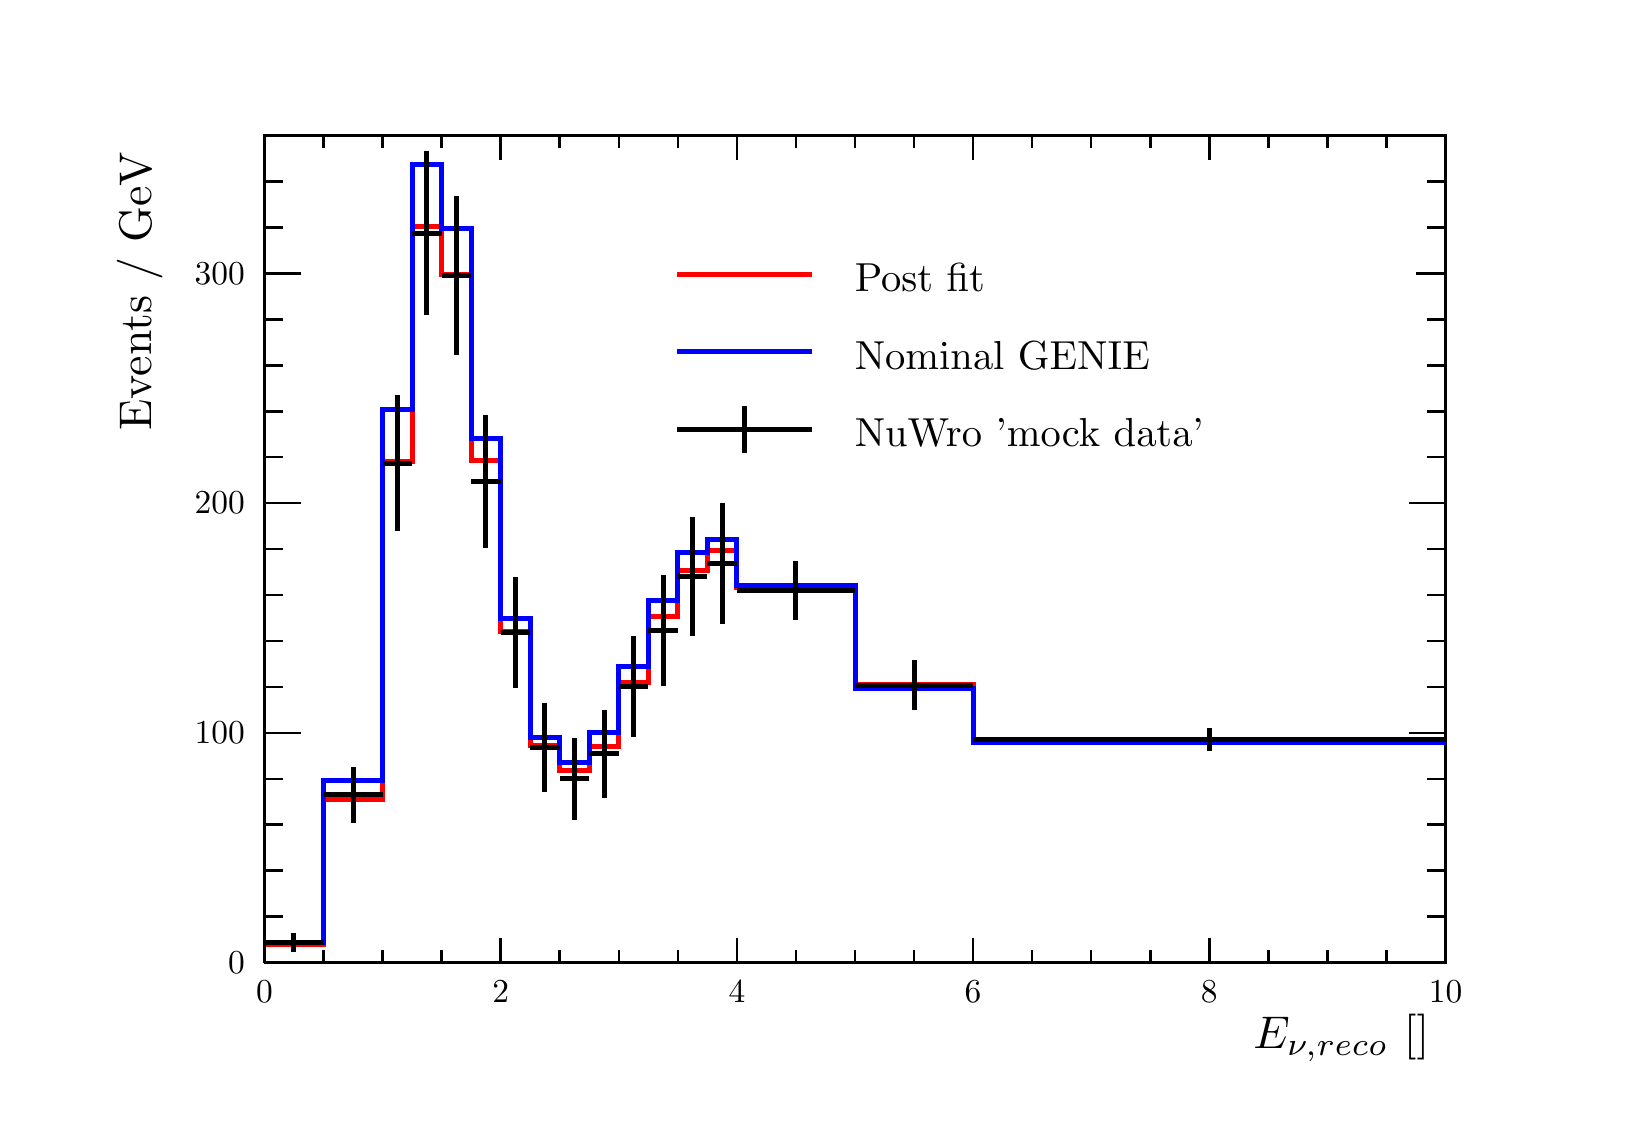
\begin{tikzpicture}
\pgfdeclareplotmark{cross} {
\pgfpathmoveto{\pgfpoint{-0.3\pgfplotmarksize}{\pgfplotmarksize}}
\pgfpathlineto{\pgfpoint{+0.3\pgfplotmarksize}{\pgfplotmarksize}}
\pgfpathlineto{\pgfpoint{+0.3\pgfplotmarksize}{0.3\pgfplotmarksize}}
\pgfpathlineto{\pgfpoint{+1\pgfplotmarksize}{0.3\pgfplotmarksize}}
\pgfpathlineto{\pgfpoint{+1\pgfplotmarksize}{-0.3\pgfplotmarksize}}
\pgfpathlineto{\pgfpoint{+0.3\pgfplotmarksize}{-0.3\pgfplotmarksize}}
\pgfpathlineto{\pgfpoint{+0.3\pgfplotmarksize}{-1.\pgfplotmarksize}}
\pgfpathlineto{\pgfpoint{-0.3\pgfplotmarksize}{-1.\pgfplotmarksize}}
\pgfpathlineto{\pgfpoint{-0.3\pgfplotmarksize}{-0.3\pgfplotmarksize}}
\pgfpathlineto{\pgfpoint{-1.\pgfplotmarksize}{-0.3\pgfplotmarksize}}
\pgfpathlineto{\pgfpoint{-1.\pgfplotmarksize}{0.3\pgfplotmarksize}}
\pgfpathlineto{\pgfpoint{-0.3\pgfplotmarksize}{0.3\pgfplotmarksize}}
\pgfpathclose
\pgfusepathqstroke
}
\pgfdeclareplotmark{cross*} {
\pgfpathmoveto{\pgfpoint{-0.3\pgfplotmarksize}{\pgfplotmarksize}}
\pgfpathlineto{\pgfpoint{+0.3\pgfplotmarksize}{\pgfplotmarksize}}
\pgfpathlineto{\pgfpoint{+0.3\pgfplotmarksize}{0.3\pgfplotmarksize}}
\pgfpathlineto{\pgfpoint{+1\pgfplotmarksize}{0.3\pgfplotmarksize}}
\pgfpathlineto{\pgfpoint{+1\pgfplotmarksize}{-0.3\pgfplotmarksize}}
\pgfpathlineto{\pgfpoint{+0.3\pgfplotmarksize}{-0.3\pgfplotmarksize}}
\pgfpathlineto{\pgfpoint{+0.3\pgfplotmarksize}{-1.\pgfplotmarksize}}
\pgfpathlineto{\pgfpoint{-0.3\pgfplotmarksize}{-1.\pgfplotmarksize}}
\pgfpathlineto{\pgfpoint{-0.3\pgfplotmarksize}{-0.3\pgfplotmarksize}}
\pgfpathlineto{\pgfpoint{-1.\pgfplotmarksize}{-0.3\pgfplotmarksize}}
\pgfpathlineto{\pgfpoint{-1.\pgfplotmarksize}{0.3\pgfplotmarksize}}
\pgfpathlineto{\pgfpoint{-0.3\pgfplotmarksize}{0.3\pgfplotmarksize}}
\pgfpathclose
\pgfusepathqfillstroke
}
\pgfdeclareplotmark{newstar} {
\pgfpathmoveto{\pgfqpoint{0pt}{\pgfplotmarksize}}
\pgfpathlineto{\pgfqpointpolar{44}{0.5\pgfplotmarksize}}
\pgfpathlineto{\pgfqpointpolar{18}{\pgfplotmarksize}}
\pgfpathlineto{\pgfqpointpolar{-20}{0.5\pgfplotmarksize}}
\pgfpathlineto{\pgfqpointpolar{-54}{\pgfplotmarksize}}
\pgfpathlineto{\pgfqpointpolar{-90}{0.5\pgfplotmarksize}}
\pgfpathlineto{\pgfqpointpolar{234}{\pgfplotmarksize}}
\pgfpathlineto{\pgfqpointpolar{198}{0.5\pgfplotmarksize}}
\pgfpathlineto{\pgfqpointpolar{162}{\pgfplotmarksize}}
\pgfpathlineto{\pgfqpointpolar{134}{0.5\pgfplotmarksize}}
\pgfpathclose
\pgfusepathqstroke
}
\pgfdeclareplotmark{newstar*} {
\pgfpathmoveto{\pgfqpoint{0pt}{\pgfplotmarksize}}
\pgfpathlineto{\pgfqpointpolar{44}{0.5\pgfplotmarksize}}
\pgfpathlineto{\pgfqpointpolar{18}{\pgfplotmarksize}}
\pgfpathlineto{\pgfqpointpolar{-20}{0.5\pgfplotmarksize}}
\pgfpathlineto{\pgfqpointpolar{-54}{\pgfplotmarksize}}
\pgfpathlineto{\pgfqpointpolar{-90}{0.5\pgfplotmarksize}}
\pgfpathlineto{\pgfqpointpolar{234}{\pgfplotmarksize}}
\pgfpathlineto{\pgfqpointpolar{198}{0.5\pgfplotmarksize}}
\pgfpathlineto{\pgfqpointpolar{162}{\pgfplotmarksize}}
\pgfpathlineto{\pgfqpointpolar{134}{0.5\pgfplotmarksize}}
\pgfpathclose
\pgfusepathqfillstroke
}
\definecolor{c}{rgb}{1,1,1};
\draw [color=c, fill=c] (0,0) rectangle (20,13.639);
\draw [color=c, fill=c] (3,1.77307) rectangle (18,12.2751);
\definecolor{c}{rgb}{0,0,0};
\draw [c,line width=0.9] (3,1.77307) -- (3,12.2751) -- (18,12.2751) -- (18,1.77307) -- (3,1.77307);
\definecolor{c}{rgb}{1,1,1};
\draw [color=c, fill=c] (3,1.77307) rectangle (18,12.2751);
\definecolor{c}{rgb}{0,0,0};
\draw [c,line width=0.9] (3,1.77307) -- (3,12.2751) -- (18,12.2751) -- (18,1.77307) -- (3,1.77307);
\definecolor{c}{rgb}{1,0,0};
\draw [c,line width=1.8] (3,2.00055) -- (3.75,2.00055) -- (3.75,3.83983) -- (4.5,3.83983) -- (4.5,8.13471) -- (4.875,8.13471) -- (4.875,11.1223) -- (5.25,11.1223) -- (5.25,10.5099) -- (5.625,10.5099) -- (5.625,8.15144) -- (6,8.15144) -- (6,5.97373)
 -- (6.375,5.97373) -- (6.375,4.53302) -- (6.75,4.53302) -- (6.75,4.21336) -- (7.125,4.21336) -- (7.125,4.51529) -- (7.5,4.51529) -- (7.5,5.33347) -- (7.875,5.33347) -- (7.875,6.17023) -- (8.25,6.17023) -- (8.25,6.75361) -- (8.625,6.75361) --
 (8.625,7.00406) -- (9,7.00406) -- (9,6.53536) -- (10.5,6.53536) -- (10.5,5.30018) -- (12,5.30018) -- (12,4.60077) -- (18,4.60077);
\definecolor{c}{rgb}{0,0,0};
\draw [c,line width=0.9] (3,1.77307) -- (18,1.77307);
\draw [c,line width=0.9] (3,2.07994) -- (3,1.77307);
\draw [c,line width=0.9] (3.75,1.9265) -- (3.75,1.77307);
\draw [c,line width=0.9] (4.5,1.9265) -- (4.5,1.77307);
\draw [c,line width=0.9] (5.25,1.9265) -- (5.25,1.77307);
\draw [c,line width=0.9] (6,2.07994) -- (6,1.77307);
\draw [c,line width=0.9] (6.75,1.9265) -- (6.75,1.77307);
\draw [c,line width=0.9] (7.5,1.9265) -- (7.5,1.77307);
\draw [c,line width=0.9] (8.25,1.9265) -- (8.25,1.77307);
\draw [c,line width=0.9] (9,2.07994) -- (9,1.77307);
\draw [c,line width=0.9] (9.75,1.9265) -- (9.75,1.77307);
\draw [c,line width=0.9] (10.5,1.9265) -- (10.5,1.77307);
\draw [c,line width=0.9] (11.25,1.9265) -- (11.25,1.77307);
\draw [c,line width=0.9] (12,2.07994) -- (12,1.77307);
\draw [c,line width=0.9] (12.75,1.9265) -- (12.75,1.77307);
\draw [c,line width=0.9] (13.5,1.9265) -- (13.5,1.77307);
\draw [c,line width=0.9] (14.25,1.9265) -- (14.25,1.77307);
\draw [c,line width=0.9] (15,2.07994) -- (15,1.77307);
\draw [c,line width=0.9] (15.75,1.9265) -- (15.75,1.77307);
\draw [c,line width=0.9] (16.5,1.9265) -- (16.5,1.77307);
\draw [c,line width=0.9] (17.25,1.9265) -- (17.25,1.77307);
\draw [c,line width=0.9] (18,2.07994) -- (18,1.77307);
\draw [anchor=base] (3,1.26842) node[scale=1.20912, color=c, rotate=0]{0};
\draw [anchor=base] (6,1.26842) node[scale=1.20912, color=c, rotate=0]{2};
\draw [anchor=base] (9,1.26842) node[scale=1.20912, color=c, rotate=0]{4};
\draw [anchor=base] (12,1.26842) node[scale=1.20912, color=c, rotate=0]{6};
\draw [anchor=base] (15,1.26842) node[scale=1.20912, color=c, rotate=0]{8};
\draw [anchor=base] (18,1.26842) node[scale=1.20912, color=c, rotate=0]{10};
\draw [anchor= east] (18,0.812882) node[scale=1.65459, color=c, rotate=0]{$E_{\nu, reco}$ [\si{\GeV}]};
\draw [c,line width=0.9] (3,12.2751) -- (18,12.2751);
\draw [c,line width=0.9] (3,11.9682) -- (3,12.2751);
\draw [c,line width=0.9] (3.75,12.1216) -- (3.75,12.2751);
\draw [c,line width=0.9] (4.5,12.1216) -- (4.5,12.2751);
\draw [c,line width=0.9] (5.25,12.1216) -- (5.25,12.2751);
\draw [c,line width=0.9] (6,11.9682) -- (6,12.2751);
\draw [c,line width=0.9] (6.75,12.1216) -- (6.75,12.2751);
\draw [c,line width=0.9] (7.5,12.1216) -- (7.5,12.2751);
\draw [c,line width=0.9] (8.25,12.1216) -- (8.25,12.2751);
\draw [c,line width=0.9] (9,11.9682) -- (9,12.2751);
\draw [c,line width=0.9] (9.75,12.1216) -- (9.75,12.2751);
\draw [c,line width=0.9] (10.5,12.1216) -- (10.5,12.2751);
\draw [c,line width=0.9] (11.25,12.1216) -- (11.25,12.2751);
\draw [c,line width=0.9] (12,11.9682) -- (12,12.2751);
\draw [c,line width=0.9] (12.75,12.1216) -- (12.75,12.2751);
\draw [c,line width=0.9] (13.5,12.1216) -- (13.5,12.2751);
\draw [c,line width=0.9] (14.25,12.1216) -- (14.25,12.2751);
\draw [c,line width=0.9] (15,11.9682) -- (15,12.2751);
\draw [c,line width=0.9] (15.75,12.1216) -- (15.75,12.2751);
\draw [c,line width=0.9] (16.5,12.1216) -- (16.5,12.2751);
\draw [c,line width=0.9] (17.25,12.1216) -- (17.25,12.2751);
\draw [c,line width=0.9] (18,11.9682) -- (18,12.2751);
\draw [c,line width=0.9] (3,1.77307) -- (3,12.2751);
\draw [c,line width=0.9] (3.462,1.77307) -- (3,1.77307);
\draw [c,line width=0.9] (3.231,2.35651) -- (3,2.35651);
\draw [c,line width=0.9] (3.231,2.93996) -- (3,2.93996);
\draw [c,line width=0.9] (3.231,3.5234) -- (3,3.5234);
\draw [c,line width=0.9] (3.231,4.10684) -- (3,4.10684);
\draw [c,line width=0.9] (3.462,4.69029) -- (3,4.69029);
\draw [c,line width=0.9] (3.231,5.27373) -- (3,5.27373);
\draw [c,line width=0.9] (3.231,5.85718) -- (3,5.85718);
\draw [c,line width=0.9] (3.231,6.44062) -- (3,6.44062);
\draw [c,line width=0.9] (3.231,7.02407) -- (3,7.02407);
\draw [c,line width=0.9] (3.462,7.60751) -- (3,7.60751);
\draw [c,line width=0.9] (3.231,8.19096) -- (3,8.19096);
\draw [c,line width=0.9] (3.231,8.7744) -- (3,8.7744);
\draw [c,line width=0.9] (3.231,9.35785) -- (3,9.35785);
\draw [c,line width=0.9] (3.231,9.94129) -- (3,9.94129);
\draw [c,line width=0.9] (3.462,10.5247) -- (3,10.5247);
\draw [c,line width=0.9] (3.462,10.5247) -- (3,10.5247);
\draw [c,line width=0.9] (3.231,11.1082) -- (3,11.1082);
\draw [c,line width=0.9] (3.231,11.6916) -- (3,11.6916);
\draw [anchor= east] (2.9,1.77307) node[scale=1.20912, color=c, rotate=0]{0};
\draw [anchor= east] (2.9,4.69029) node[scale=1.20912, color=c, rotate=0]{100};
\draw [anchor= east] (2.9,7.60751) node[scale=1.20912, color=c, rotate=0]{200};
\draw [anchor= east] (2.9,10.5247) node[scale=1.20912, color=c, rotate=0]{300};
\draw [anchor= east] (1.416,12.2751) node[scale=1.65459, color=c, rotate=90]{Events / GeV};
\draw [c,line width=0.9] (18,1.77307) -- (18,12.2751);
\draw [c,line width=0.9] (17.538,1.77307) -- (18,1.77307);
\draw [c,line width=0.9] (17.769,2.35651) -- (18,2.35651);
\draw [c,line width=0.9] (17.769,2.93996) -- (18,2.93996);
\draw [c,line width=0.9] (17.769,3.5234) -- (18,3.5234);
\draw [c,line width=0.9] (17.769,4.10684) -- (18,4.10684);
\draw [c,line width=0.9] (17.538,4.69029) -- (18,4.69029);
\draw [c,line width=0.9] (17.769,5.27373) -- (18,5.27373);
\draw [c,line width=0.9] (17.769,5.85718) -- (18,5.85718);
\draw [c,line width=0.9] (17.769,6.44062) -- (18,6.44062);
\draw [c,line width=0.9] (17.769,7.02407) -- (18,7.02407);
\draw [c,line width=0.9] (17.538,7.60751) -- (18,7.60751);
\draw [c,line width=0.9] (17.769,8.19096) -- (18,8.19096);
\draw [c,line width=0.9] (17.769,8.7744) -- (18,8.7744);
\draw [c,line width=0.9] (17.769,9.35785) -- (18,9.35785);
\draw [c,line width=0.9] (17.769,9.94129) -- (18,9.94129);
\draw [c,line width=0.9] (17.538,10.5247) -- (18,10.5247);
\draw [c,line width=0.9] (17.538,10.5247) -- (18,10.5247);
\draw [c,line width=0.9] (17.769,11.1082) -- (18,11.1082);
\draw [c,line width=0.9] (17.769,11.6916) -- (18,11.6916);
\definecolor{c}{rgb}{0,0,1};
\draw [c,line width=1.8] (3,2.02374) -- (3.75,2.02374) -- (3.75,4.08632) -- (4.5,4.08632) -- (4.5,8.80134) -- (4.875,8.80134) -- (4.875,11.9024) -- (5.25,11.9024) -- (5.25,11.0999) -- (5.625,11.0999) -- (5.625,8.42754) -- (6,8.42754) -- (6,6.14527)
 -- (6.375,6.14527) -- (6.375,4.63331) -- (6.75,4.63331) -- (6.75,4.31774) -- (7.125,4.31774) -- (7.125,4.68858) -- (7.5,4.68858) -- (7.5,5.53271) -- (7.875,5.53271) -- (7.875,6.3761) -- (8.25,6.3761) -- (8.25,6.97785) -- (8.625,6.97785) --
 (8.625,7.14453) -- (9,7.14453) -- (9,6.5642) -- (10.5,6.5642) -- (10.5,5.25748) -- (12,5.25748) -- (12,4.56447) -- (18,4.56447);
\definecolor{c}{rgb}{0,0,0};
\draw [c,line width=1.8] (3.375,1.90119) -- (3.375,2.02162);
\draw [c,line width=1.8] (3.375,2.02162) -- (3.375,2.14204);
\draw [c,line width=1.8] (3,2.02162) -- (3.375,2.02162);
\draw [c,line width=1.8] (3.375,2.02162) -- (3.75,2.02162);
\foreach \P in {(3.375,2.02162)}{\draw[mark options={color=c,fill=c},mark size=2.402402pt, line width=0.000000pt, mark=*,mark size=1pt] plot coordinates {\P};}
\draw [c,line width=1.8] (4.125,3.55166) -- (4.125,3.90429);
\draw [c,line width=1.8] (4.125,3.90429) -- (4.125,4.25692);
\draw [c,line width=1.8] (3.75,3.90429) -- (4.125,3.90429);
\draw [c,line width=1.8] (4.125,3.90429) -- (4.5,3.90429);
\foreach \P in {(4.125,3.90429)}{\draw[mark options={color=c,fill=c},mark size=2.402402pt, line width=0.000000pt, mark=*,mark size=1pt] plot coordinates {\P};}
\draw [c,line width=1.8] (4.6875,7.25437) -- (4.6875,8.1146);
\draw [c,line width=1.8] (4.6875,8.1146) -- (4.6875,8.97482);
\draw [c,line width=1.8] (4.5,8.1146) -- (4.6875,8.1146);
\draw [c,line width=1.8] (4.6875,8.1146) -- (4.875,8.1146);
\foreach \P in {(4.6875,8.1146)}{\draw[mark options={color=c,fill=c},mark size=2.402402pt, line width=0.000000pt, mark=*,mark size=1pt] plot coordinates {\P};}
\draw [c,line width=1.8] (5.0625,9.99505) -- (5.0625,11.0346);
\draw [c,line width=1.8] (5.0625,11.0346) -- (5.0625,12.0742);
\draw [c,line width=1.8] (4.875,11.0346) -- (5.0625,11.0346);
\draw [c,line width=1.8] (5.0625,11.0346) -- (5.25,11.0346);
\foreach \P in {(5.0625,11.0346)}{\draw[mark options={color=c,fill=c},mark size=2.402402pt, line width=0.000000pt, mark=*,mark size=1pt] plot coordinates {\P};}
\draw [c,line width=1.8] (5.4375,9.48462) -- (5.4375,10.4934);
\draw [c,line width=1.8] (5.4375,10.4934) -- (5.4375,11.5021);
\draw [c,line width=1.8] (5.25,10.4934) -- (5.4375,10.4934);
\draw [c,line width=1.8] (5.4375,10.4934) -- (5.625,10.4934);
\foreach \P in {(5.4375,10.4934)}{\draw[mark options={color=c,fill=c},mark size=2.402402pt, line width=0.000000pt, mark=*,mark size=1pt] plot coordinates {\P};}
\draw [c,line width=1.8] (5.8125,7.03813) -- (5.8125,7.88247);
\draw [c,line width=1.8] (5.8125,7.88247) -- (5.8125,8.7268);
\draw [c,line width=1.8] (5.625,7.88247) -- (5.8125,7.88247);
\draw [c,line width=1.8] (5.8125,7.88247) -- (6,7.88247);
\foreach \P in {(5.8125,7.88247)}{\draw[mark options={color=c,fill=c},mark size=2.402402pt, line width=0.000000pt, mark=*,mark size=1pt] plot coordinates {\P};}
\draw [c,line width=1.8] (6.1875,5.26461) -- (6.1875,5.96391);
\draw [c,line width=1.8] (6.1875,5.96391) -- (6.1875,6.66321);
\draw [c,line width=1.8] (6,5.96391) -- (6.1875,5.96391);
\draw [c,line width=1.8] (6.1875,5.96391) -- (6.375,5.96391);
\foreach \P in {(6.1875,5.96391)}{\draw[mark options={color=c,fill=c},mark size=2.402402pt, line width=0.000000pt, mark=*,mark size=1pt] plot coordinates {\P};}
\draw [c,line width=1.8] (6.5625,3.94327) -- (6.5625,4.50822);
\draw [c,line width=1.8] (6.5625,4.50822) -- (6.5625,5.07316);
\draw [c,line width=1.8] (6.375,4.50822) -- (6.5625,4.50822);
\draw [c,line width=1.8] (6.5625,4.50822) -- (6.75,4.50822);
\foreach \P in {(6.5625,4.50822)}{\draw[mark options={color=c,fill=c},mark size=2.402402pt, line width=0.000000pt, mark=*,mark size=1pt] plot coordinates {\P};}
\draw [c,line width=1.8] (6.9375,3.58321) -- (6.9375,4.10483);
\draw [c,line width=1.8] (6.9375,4.10483) -- (6.9375,4.62645);
\draw [c,line width=1.8] (6.75,4.10483) -- (6.9375,4.10483);
\draw [c,line width=1.8] (6.9375,4.10483) -- (7.125,4.10483);
\foreach \P in {(6.9375,4.10483)}{\draw[mark options={color=c,fill=c},mark size=2.402402pt, line width=0.000000pt, mark=*,mark size=1pt] plot coordinates {\P};}
\draw [c,line width=1.8] (7.3125,3.8659) -- (7.3125,4.42185);
\draw [c,line width=1.8] (7.3125,4.42185) -- (7.3125,4.9778);
\draw [c,line width=1.8] (7.125,4.42185) -- (7.3125,4.42185);
\draw [c,line width=1.8] (7.3125,4.42185) -- (7.5,4.42185);
\foreach \P in {(7.3125,4.42185)}{\draw[mark options={color=c,fill=c},mark size=2.402402pt, line width=0.000000pt, mark=*,mark size=1pt] plot coordinates {\P};}
\draw [c,line width=1.8] (7.6875,4.63705) -- (7.6875,5.27643);
\draw [c,line width=1.8] (7.6875,5.27643) -- (7.6875,5.91581);
\draw [c,line width=1.8] (7.5,5.27643) -- (7.6875,5.27643);
\draw [c,line width=1.8] (7.6875,5.27643) -- (7.875,5.27643);
\foreach \P in {(7.6875,5.27643)}{\draw[mark options={color=c,fill=c},mark size=2.402402pt, line width=0.000000pt, mark=*,mark size=1pt] plot coordinates {\P};}
\draw [c,line width=1.8] (8.0625,5.2864) -- (8.0625,5.98768);
\draw [c,line width=1.8] (8.0625,5.98768) -- (8.0625,6.68896);
\draw [c,line width=1.8] (7.875,5.98768) -- (8.0625,5.98768);
\draw [c,line width=1.8] (8.0625,5.98768) -- (8.25,5.98768);
\foreach \P in {(8.0625,5.98768)}{\draw[mark options={color=c,fill=c},mark size=2.402402pt, line width=0.000000pt, mark=*,mark size=1pt] plot coordinates {\P};}
\draw [c,line width=1.8] (8.4375,5.92403) -- (8.4375,6.68078);
\draw [c,line width=1.8] (8.4375,6.68078) -- (8.4375,7.43754);
\draw [c,line width=1.8] (8.25,6.68078) -- (8.4375,6.68078);
\draw [c,line width=1.8] (8.4375,6.68078) -- (8.625,6.68078);
\foreach \P in {(8.4375,6.68078)}{\draw[mark options={color=c,fill=c},mark size=2.402402pt, line width=0.000000pt, mark=*,mark size=1pt] plot coordinates {\P};}
\draw [c,line width=1.8] (8.8125,6.07294) -- (8.8125,6.84203);
\draw [c,line width=1.8] (8.8125,6.84203) -- (8.8125,7.61111);
\draw [c,line width=1.8] (8.625,6.84203) -- (8.8125,6.84203);
\draw [c,line width=1.8] (8.8125,6.84203) -- (9,6.84203);
\foreach \P in {(8.8125,6.84203)}{\draw[mark options={color=c,fill=c},mark size=2.402402pt, line width=0.000000pt, mark=*,mark size=1pt] plot coordinates {\P};}
\draw [c,line width=1.8] (9.75,6.12584) -- (9.75,6.49706);
\draw [c,line width=1.8] (9.75,6.49706) -- (9.75,6.86829);
\draw [c,line width=1.8] (9,6.49706) -- (9.75,6.49706);
\draw [c,line width=1.8] (9.75,6.49706) -- (10.5,6.49706);
\foreach \P in {(9.75,6.49706)}{\draw[mark options={color=c,fill=c},mark size=2.402402pt, line width=0.000000pt, mark=*,mark size=1pt] plot coordinates {\P};}
\draw [c,line width=1.8] (11.25,4.97434) -- (11.25,5.29487);
\draw [c,line width=1.8] (11.25,5.29487) -- (11.25,5.6154);
\draw [c,line width=1.8] (10.5,5.29487) -- (11.25,5.29487);
\draw [c,line width=1.8] (11.25,5.29487) -- (12,5.29487);
\foreach \P in {(11.25,5.29487)}{\draw[mark options={color=c,fill=c},mark size=2.402402pt, line width=0.000000pt, mark=*,mark size=1pt] plot coordinates {\P};}
\draw [c,line width=1.8] (15,4.46209) -- (15,4.60582);
\draw [c,line width=1.8] (15,4.60582) -- (15,4.74956);
\draw [c,line width=1.8] (12,4.60582) -- (15,4.60582);
\draw [c,line width=1.8] (15,4.60582) -- (18,4.60582);
\foreach \P in {(15,4.60582)}{\draw[mark options={color=c,fill=c},mark size=2.402402pt, line width=0.000000pt, mark=*,mark size=1pt] plot coordinates {\P};}
\definecolor{c}{rgb}{1,1,1};
\draw [color=c, fill=c] (2,12.8206) rectangle (18,13.5708);
\definecolor{c}{rgb}{0,0,0};
%\draw (10,13.1957) node[scale=1.40004, color=c, rotate=0]{$\nu_{\mu} RHC postfit: \delta = 1.57, \chi^{2} = 2.33$};
\definecolor{c}{rgb}{1,1,1};
\draw [color=c, fill=c] (7.87966,8.05158) rectangle (17.6218,11.0029);
\definecolor{c}{rgb}{0,0,0};
\draw [anchor=base west] (10.3152,10.2896) node[scale=1.46368, color=c, rotate=0]{Post fit};
\definecolor{c}{rgb}{1,0,0};
\draw [c,line width=1.8] (8.24499,10.511) -- (9.94986,10.511);
\definecolor{c}{rgb}{0,0,0};
\draw [anchor=base west] (10.3152,9.30587) node[scale=1.46368, color=c, rotate=0]{Nominal GENIE};
\definecolor{c}{rgb}{0,0,1};
\draw [c,line width=1.8] (8.24499,9.52722) -- (9.94986,9.52722);
\definecolor{c}{rgb}{0,0,0};
\draw [anchor=base west] (10.3152,8.32211) node[scale=1.46368, color=c, rotate=0]{NuWro 'mock data'};
\draw [c,line width=1.8] (8.24499,8.54346) -- (9.94986,8.54346);
\draw [c,line width=1.8] (9.09742,8.24833) -- (9.09742,8.83859);
\end{tikzpicture}
